\section{Ranking Algorithms}
\label{sec:rankingAlgorithms}
When a search is done on our search-engine, the method \code{getMachingQueries} in \code{QueryHandler} finds all the websites that matches the query. But of course some of the matching websites are more relevant than others, for the given query. To show the user the most relevant pages at the top, we need a way to rank the websites according to relevance, i.e we need a ranking algorithm. There are many different ways to rank a website, we have chosen to implement the term-frequency algorithm (TF-algorithm), the term-frequency inverse-document-frequency (TFIDF-algorithm), and also our own  term-frequency inverse-corpus-frequency (TFICF-algorithm).    

\subsection{Term Frequency}
Keeping in line with the notation at \cite{wikiTFIDF} the term frequency, TF, is calculated as follows.

\[ TF = \frac{f_{t,d}}{\sum_{i \in d}f_{i,d}} \]

Note that we have choosen the term frequency that is weighted by the total number of words in the document/site. %The corresponding Java implementation is shown in listing \ref{lst:tf}.




\subsection{Term Frequency - Inverse \emph{Corpus} Frequency}
Instead of using the inverse document frequency as above, it would also be sensible to use the \emph{inverse term frequency} with respect to the whole database/corpus. Lets call that algorithm for TFICF (Term frequency - Inverse Corpus Frequency).
    
\[ TFICF = TF \cdot \log{\left( \frac{C_{total}}{C_{word}} \right) } \]

Where \(C_{total}\) is the total number of words in the corpus (duplicates allowed), and \(C_{word}\) is the number of times the specific word appears in the corpus. 



\subsection{Comparison of Algorithms}
TFIDF and TFICF are conceptually almost identical, but they are conceptually quite different from the TF algorithm. 

TF algorithm only counts how often a word appers on a site. So lets say that you search for a fairly common word like "government", and a relatively rare word like "Togo". Then you risk that the government word gets many hits compared to "Togo" even on a site about The goverment of Togo. And since the rare word doesn't contribute significantly to the score, sites about governments might be ranked to high compared to sites about Togo. 
This effect will be larger if the TF implementation only uses the word count and not the word frequency as we do. The described effect can still be seen as shown in table \ref{tab:comparisonRankingAlgorithms}, but the TF algorithm is actually quite good in most cases we tried out.   
TFIDF (and our TFICF) takes into account the rarity of words by weighing them according to how common/rare they are in the corpus of websites. 
Togo doesn't appear very often in the corpus (38 occourrences in medium database), and therefore even if a site has just a few occurrences of "Togo" the search word counts for more than many occurrences of the word "government" (which appears 3067 times in the medium database.
This is a reasonable behavior since the rare words are probably the best indicators of what the user really wants to read about.  

\begin{table}[b]
	\centering
\begin{tabular}{@{}llr@{}} \toprule
	\multicolumn{3}{c}{Search query: \textit{Togo OR Government}} \\ \cmidrule(r){1-3}
	TF 									& TFIDF 							& TFICF \\ \midrule
	Prime Minister of Spain 			& Economy of Togo 					& Economy of Togo \\
	Caretaker government 				& Prime Minister of Spain 			& Prime Minister of Spain \\
	Economy of Togo		    			& Caretaker government 				& Caretaker government \\
	State government 					& State government					& State government \\
	Government of the UK 	& Government of the UK 	& Government of the UK \\ \bottomrule
\end{tabular}
\caption{Top 5 results for different ranking algorithms.}	
\label{tab:comparisonRankingAlgorithms}
\end{table}


\subsection{Design considerations}
In this section we will describe how we chose to embed/implement ranking algorithms in our search-engine. We actually have two different working implementations, and there was a passionate group discussion about which implementation to chose for our search-engine.  

A common rule of thumb for deciding on how to distribute responsibility between classes and methods in a program, is to say that methods correspond to verbs, and classes to nouns. This verb/noun method is described in \cite[p.530]{BK}.
But what kind of word is `rank` or `score`, a verb or a noun? Actually it can be both, and this suggests that we can implement a ranking algorithm using different design styles.

\subsubsection{Option 1: Score as Utility Class}
\begin{figure}[t]
	\centering
	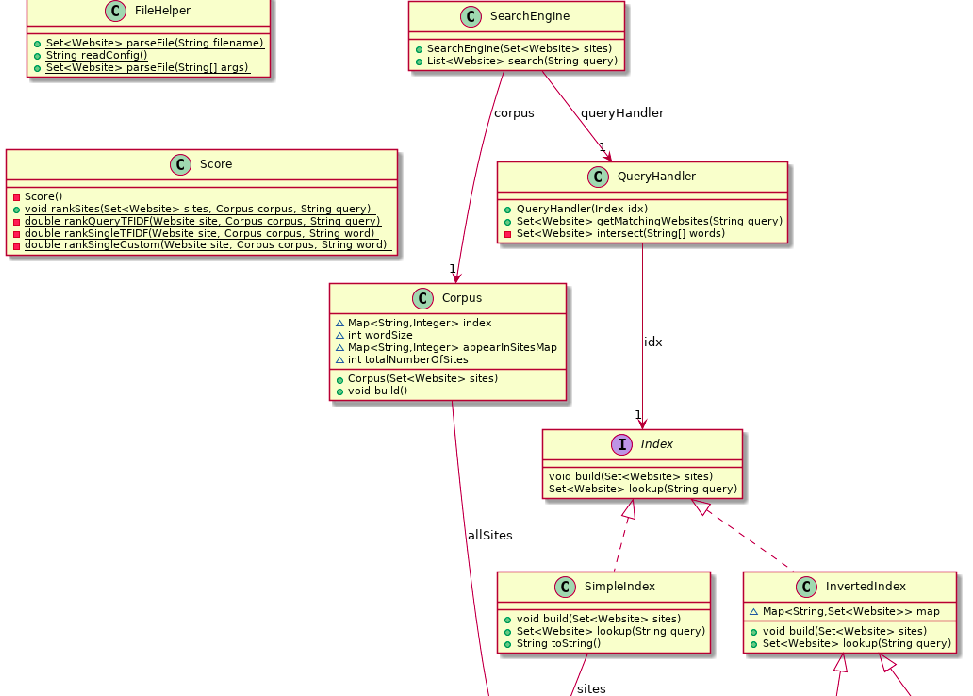
\includegraphics[width=\textwidth]{graphics/uml/ScoreAsUtilityZoom.png}
	\caption{UML Diagram for the search-engine when Score is a utility class.}
	\label{fig:uml:ScoreAsUtility}
\end{figure}

In the first implementation we tried, we wrote a utility class named \code{Score} which had static rank methods for ranking websites.   
A (relevant part of the) UML class diagram for this design is shown in figure \ref{fig:uml:ScoreAsClass}, and snippets of relevant code lines from the implementation is shown in listing \ref{lst:ScoreUtilityClass} and \ref{lst:ScoreUtilityClass-2}. 
A drawback of this method is that it doesn't have a \code{Score} interface as specified in the mandatory requirements for the assignment.
Another drawback of this implementation is that the ranking methods works by having a sideeffect, rather than returning a value. The ranking methods sets a score field in the website. This field is then used when sorting the sites. A better way would be to make ranking methods with no sideeffect and instead return the website score directly, and use this for sorting. This is fixed in the second implementation we did.      

\begin{lstlisting}[language={Java}, caption={Snippet from the Score utility class.}, label={lst:ScoreUtilityClass}]
//// From Score class 

/**
* Rank the sites according to the whole query. I.e calculate and set the rank field of each
* website in the supplied set. The ranking algorithm we have chosen is TFIDF.
* 
* @param sites a set of websites that are to be ranked.
* @param corpus the corpus of all websites.
* @param query the searh query.
* 
* @return the method has no return value. But the methods side effect is to set the rank field
*         for the supplied set of websites.
*/
public static void rankSites(Set<Website> sites, Corpus corpus, String query) {
	for (Website site : sites) {
		site.setRank(rankQueryTFIDF(site, corpus, query)); 
		// bad decision! 
		// better just to use double from rankQueryTFIDF() and do the sorting imidiately. 
	}
}
\end{lstlisting}

\begin{lstlisting}[language={Java}, caption={Snippets from SearchEngine and Website, from the first implementation where Score was a utility class.}, label={lst:ScoreUtilityClass-2}]
//// From SearchEngine 

	Set<Website> results = queryHandler.getMatchingWebsites(query);
	
	// rank the websites that matches the query
	Score.rankSites(results, this.corpus, query); // using the static method Score.rankSites.
	
	// OBS: convert a set of websites to a list, since the sort method only works for list.
	List<Website> resultList = results.stream().collect(Collectors.toList());  
	
	// make a Comparator from the static method Comparator.comparingDouble()
	Comparator<Website> rankComparator = Comparator.comparingDouble(Website::getRank);
	resultList.sort(rankComparator.reversed()); 

//// From Website

	/**
	*  Set the rank of the site. This method is used by an external ranking method
	* to set the rank of the site. 
	* 
	* @param rank the rank that is to be assigned to the website.  
	*/
	public void setRank(double rank) {
		this.rank = rank;
	}

	/**
	* Returns the currently assigned rank of the website. 
	* 
	* @return the current rank of the website. 
	*/
	public double getRank() {
		return rank;
	}
\end{lstlisting}


\subsubsection{Option 2: Score as Interface}
\begin{sidewaysfigure}[t]
%\begin{figure}[t]
	\centering
	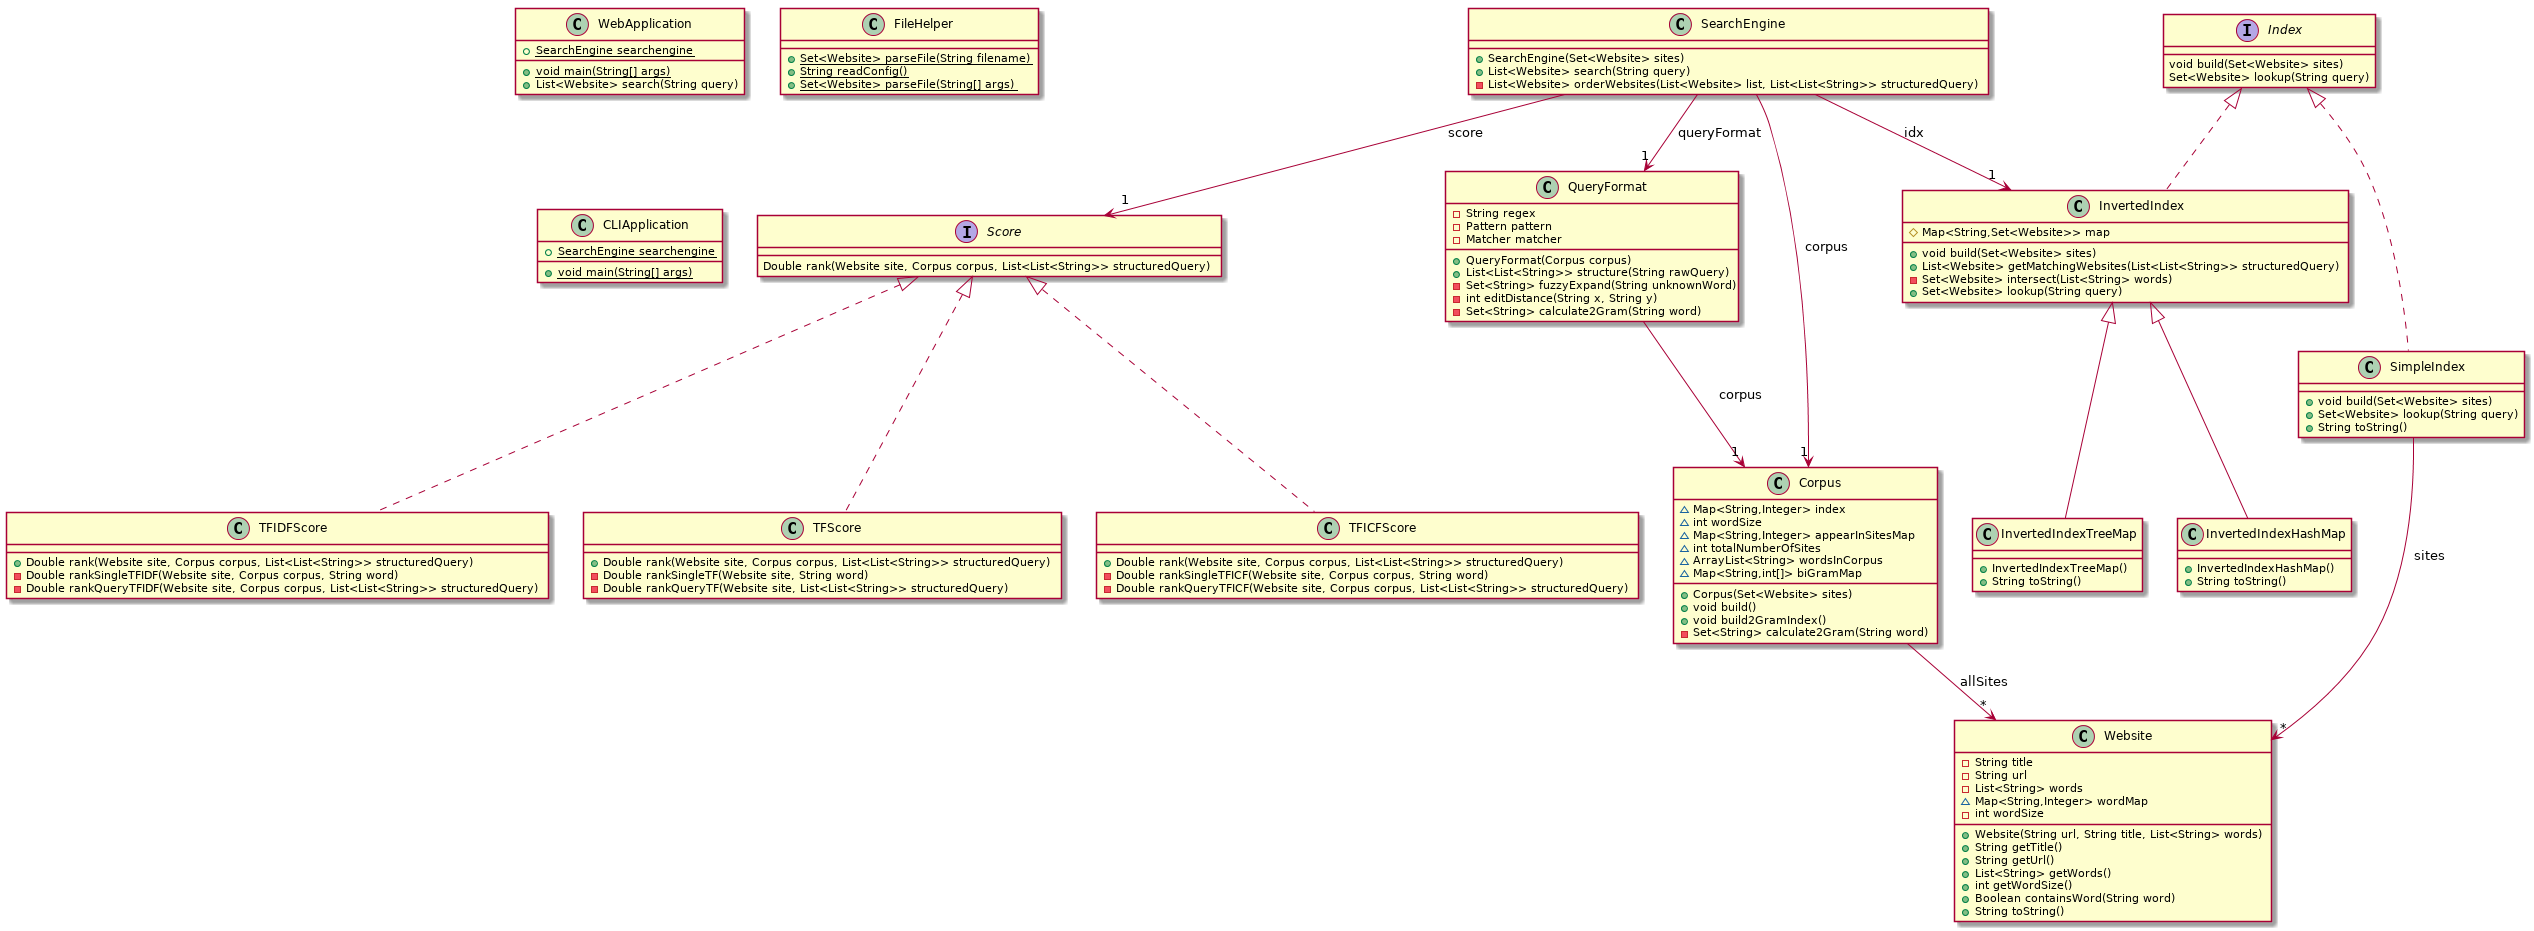
\includegraphics[width=\textwidth]{graphics/uml/ScoreAsInterface.png}
	\caption{UML Diagram for search-engine when using an interface Score.}
	\label{fig:uml:ScoreAsInterface}
%\end{figure}
\end{sidewaysfigure}
Another option which largely preserves the same division of responsibility is shown in the class diagram in figure \ref{fig:uml:ScoreAsInterface}. This is the solution we went with in our final version of the code. Relevant coding lines from the implementation is shown in listing \ref{lst:scoreInterface}.
This solution has the \code{Score} interface as required, and another big improvement is that the rank field from \code{Website} is removed, and instead we use the value from \code{rank} method directly to do the sorting.  


\begin{lstlisting}[language={Java}, caption={Final implementation where Score is an interface.}, label={lst:scoreInterface}]
//// From TFIDFScore class 

// Rank the site according to the whole query, and the Corpus.
@Override
public Double rank(Website site, Corpus corpus, String query) {
	return rankQueryTFIDF(site, corpus, query);
}


//// From SearchEngine 

/**
* Rank a list of websites, according to the query, 
* also using information about the whole database from corpus object. 
*
* @param list List of websites to be ordered according to rank.
* @param query The search query.
* @return return the list of websites reordered according to rank.
* I.e the method modifies the input list.  
*/
private List<Website> orderWebsites(List<Website> list, String query) {
	// create a nested Comparator class
	class RankComparator implements Comparator<Website> {
		public int compare(Website site, Website otherSite) {
			return score.rank(site, corpus, query).compareTo(score.rank(otherSite, corpus, query));
		}
	}

	// sort the websites according to their rank.
	list.sort(new RankComparator().reversed());     
	return list;
}
\end{lstlisting}



